\documentclass[12pt,letterpaper, onecolumn]{exam}
\usepackage{amsmath}
\usepackage{amssymb}
\usepackage[lmargin=71pt, tmargin=1.2in]{geometry}
\usepackage{graphicx}%For centering solution box
\lhead{IND ENG 221\\}
\rhead{Kartikeya Sharma\\}
% \chead{\hline} % Un-comment to draw line below header
\thispagestyle{empty}   %For removing header/footer from page 1

\begin{document}

\begingroup  
    \centering
    \LARGE IND ENG 221\\
    \LARGE HW 1\\[0.5em]
    \large \today\\[0.5em]
    \large Kartikeya Sharma\par
    \large SID: 3037376860\par
\endgroup
\rule{\textwidth}{0.4pt}
\pointsdroppedatright   %Self-explanatory
\printanswers
\renewcommand{\solutiontitle}{\noindent\textbf{Ans:}\enspace}   %Replace "Ans:" with starting keyword in solution box

\begin{questions}

    \question What is the monthly payment for a 5 year car loan of \$ 20,000with 10\% fixed interest rate (monthly compounding)? Assume 5 x 12 = 60 equal monthly payments
    
    \begin{solution}
        
    \end{solution}
    
    \question Suppose that the 6-month, 12-month, 18-month, and 24-month zero rates are 5\%, 6\%, 6.5\%, and 7\%, respectively, with semiannual compounding. What is the 2-year par yield? (The par yield for a certain bond maturity is the coupon rate that causes the bond price to equal its par value (= the notional value.). Assume the bond pays coupon semi-annually. (Hull 4.22)

    \begin{solution}
            
    \end{solution}

    \pagebreak %Not necessary
    
    \question Suppose that risk-free zero interest rates with continuous compounding are as above:
    Calculate forward interest rates for the second, third, fourth, and fifth years. (Hull 4.23)
    
    \begin{figure}
        \centering
        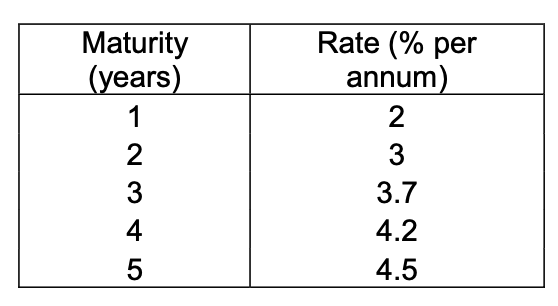
\includegraphics[width=.5\linewidth]{tbl.png}
        \caption{tbl}
        \label{fig:enter-label}
    \end{figure}

    \begin{solution}
            
    \end{solution}

    \question The cash prices of 6-month and 1-year Treasury bills are 94.0 and 89.0. A 1.5-year Treasury bond that will pay coupons of \$4 every 6 months currently sells for \$94.84. A 2-year Treasury bond that will pay coupons of \$5 every 6 months currently sells for \$97.12.Calculate the 6-month, 1-year, 1.5-year, and 2-year Treasury zero rates. (Hull 4.29)

    \begin{solution}
            
    \end{solution}

    \question An interest rate is quoted as 5\% per annum with semiannual compounding. What is the equivalent rate with (a) annual compounding, (b) monthly compounding, and (c) continuous compounding. (Hull 4.34)

    \begin{solution}
            
    \end{solution}

    
\end{questions}
\end{document}